\chapter{Mikrodenetleyicilerin Programlanması}

\acrfull{MCU}, içerisinde hafıza birimleri(RAM, ROM, Flash), giriş/çıkış birimleri olan programlanabilen entegrelerdir.
%%-_--_-_-_-_-_-_-_-_-_-_-_-_-_-_-_-Denetleyici Resimi Koy-_-_-_-_-_-_-_-_-_-_-_-_-_-_-_-_-_-_-_-_-_-_-_

\begin{figure}[h]
\centering
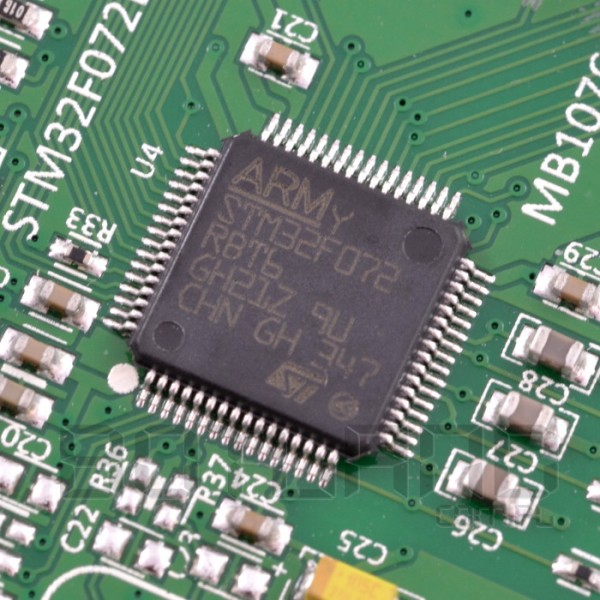
\includegraphics[width=0.6\textwidth]{gorseller/mcu}
\caption{STM32F Serisi Mikrodenetleyici}\label{fig:mcu}
\end{figure}

Mikrodenetleyicilerin programlanması, bilgisayar oramında yazılmış olan kodun hedef işlemci için derlenmesi ve derleme sonucu ortaya çıkan makina kodlarının bir şekilde denetleyicinin hafıza birimine aktarılması olarak açıklanır. Mikrodenetlecilerden önce mikroişlemciler ile kurulan sistemlerde programlama işlemi, hafıza biriminin sistemden ayırarak bir programlayıcı yardımı ile makina kodlarının aktarılmasıyla gerçekleşiyordu. Mikrodenetleyicilerde hafıza birimi entegre içinde gömülü olarak bulunduğu için programalama işlemini bu şekilde gerçeklemek mümkün değildir.

Günümüzde mikrodenetleyiciler \acrfull{ICSP} olarak adlandırılan programlayıcılar ile programlanmaktadır. \acrshort{ICSP} programlayıcılar, denetleyicinin programlama pinleri aracılığıyla işlemcinin hafıza birimine erişim sağlayarak makina kodlarını aktarır. Bu işlem ARM tabanlı mikrodenetleyicilerde \acrfull{SWD} debug portu ya da JTAG portu ile gerçekleştirmektedir.
